O processamento de linguagem natural (NLP), é um dos principais ramos da Inteligência Artificial.
Um dos marcos inicias desta área de conhecimento foi o teste de Turing~\cite{turing50} no qual a capacidade
de comunicação é proposta como um critério de inteligência.
Desde sua criação, no inicio dos anos 50, o NLP se consolidou de maneira a estar presente no dia a dia das pessoas como
se observa na utilização de serviços automatizados de atendimento ao clientes, ferramentas de tradução, e outros.
Grande parte destas aplicações provém da utilização de técnicas de aprendizado supervisionado que serão apresentadas
no Capítulo~\ref{supervisionado}.

A Figura~\ref{fig:pipeline} apresenta o diagrama de blocos contendo todas as etapas de um classificador de análise de
sentimento de \textit{tweets}.
As seções a seguir apresentam as transformações aplicadas a textos necessárias para viabilizar a aplicação de algoritmos
de aprendizado, estes são os processos que formam as duas primeiras etapas do classificador como descrito na imagem.

\begin{figure}
\begin{center} {
    \begin{center}
    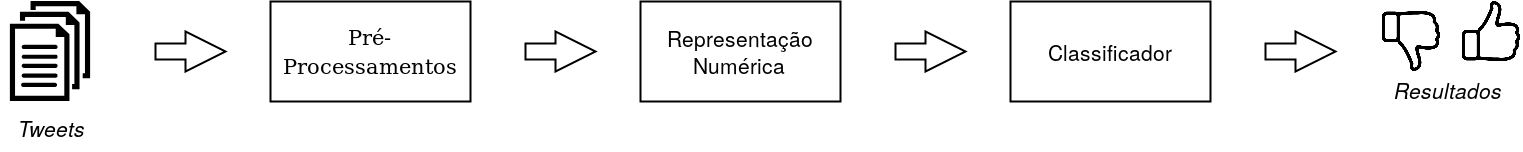
\includegraphics[scale=0.275]{pipeline.png}
    \caption{Diagrama de blocos de classificador de análise de sentimento.}
    \label{fig:pipeline}
    \end{center}
}
\end{center}
\end{figure}

\section{Pré-processamentos}

A primeira etapa na preparação de uma mensagem para utilização em algoritmos de aprendizado de máquina é a separação por
palavras.
Este processo é chamado de \textit{tokenização}, denominando-se cada palavra resultante como um token.
A \textit{tokenização} costuma incluir a separação de contrações como a transformação de \textit{dela} em \textit{de}
e \textit{ela}.

% figura mostrando tokenização

Para aplicação de tarefas como classificação, é comum se remover as palavras mais comuns de um idioma e que não
agregam informação discriminante para o objetivo desejado, essas palavras são chamadas de \textit{stopwords}.
A remoção de \textit{stopwords} visa reduzir o ruído presente em dados textuais, aumentando a acurácia dos algoritmos de
aprendizado de máquina e reduzindo a complexidade do problema~\cite{silva03}.
Porém, a remoção de \textit{stopwords} provindas de listas pré compiladas, técnica mais utilizada, apresenta desafios
devido a dinamicidade de meios como redes sociais.
Saif \textit{et al.}~\cite{saif14} apresentam um estudo comparativo da remoção de \textit{stopwords} por diferentes
técnicas e seus efeitos na classificação de sentimento de \textit{tweets}.
Além da remoção de \textit{stopwords}, em mensagens provindas de redes sociais também são costumeiramente removidos
links, \textit{hashtags} e menções a usuários.

Também é possível realizar a correção ortográfica das palavras e a lematização, processo de extração do radical da
palavra.
Estas técnicas são normalmente empregadas para reduzir o vocabulário e diminuir assim a complexidade do treinamento.

\section{Representações Numéricas}

Contudo, a utilização de algoritmos de aprendizado de máquina depende de uma representação numérica dos dados.
Após a conversão de uma mensagem em uma uma sequência de tokens, há uma etapa de transformação destas cadeias
de tokens em matrizes ou vetores.
Serão apresentadas nas subseções seguintes as principais técnicas referentes a este processo.

\subsection{Codificação One-Hot}

Um dos métodos mais observados na literatura é a codificação \textit{one-hot}, na qual cada token é representado de
maneira maximamente esparsa.
Ou seja, é definido um espaço cujo número de dimensão é dada pelo tamanho do vocabulário utilizado e cada palavra é
substituída por um vetor unitário na direção que representa sua posição no vocabulário.
Desta maneira, cada token é representado por um vetor unitário de dimensão igual a do vocabulário.

Outra forma possível de utilização é transformar cada par de palavras em um token.
A utilização de múltiplas palavras por token é chamada de \textit{n-gram}.
A ideia da aplicação de \textit{n-gram} é capturar expressões ou distinguir palavras em diferentes contextos.
Porém, sua utilização aumenta significativamente o tamanho do vocabulário, podendo dificultar o processo de treinamento.

\subsection{Bag-of-Words}

Uma vez que cada palavra é caracterizada por sua codificação \textit{one-hot}, a forma natural de simbolizar uma mensagem
é por uma matriz na qual cada coluna é composta pelo vetor correspondente a cada palavra da frase.
Contudo, para evitar o aumento da dimensionalidade do problema é comum se utilizar da técnica \textit{bag-of-words} na
qual cada mensagem é representada pela soma dos vetores de seus tokens~\cite{schutze08}.

Esta técnica também é chamada na literatura como \textit{term frequence} (tf), dado que a técnica é dada pela contagem
de termos de um documento.
Nesse caso as palavras são pesadas igualmente, outra abordagem possível é multiplicar a frequência do termo no documento
pelo inverso do número de documentos no qual aquele termo aparece, técnica denominada \textit{term frequence-inverse
document frequence} (TF-IDF)~\cite{salton88}.
A TF-IDF permite compensar a grande presença de palavras muito frequentes, que limitariam a influência de termos pouco
usados.

É possível notar que a utilização de ambas as técnicas ignora a ordem das palavras na frase.
Técnicas como Word2Vec, apresentada na Seção~\ref{sec:w2v}, permitem a utilização da posição do termo na mensagem por conter
uma representação densa de cada token, reduzindo a dimensionalidade do problema.

\subsection{Word2Vec} \label{sec:w2v}

Word2Vec~\cite{mikolov13} (W2V) é uma técnica que visa representar uma palavra por um vetor de números reais, denso e de
tamanho arbitrário.
Os resultados obtidos por Mikolov \textit{et at.}~\cite{mikolov13} mostram que a representação vetorial é capaz de
capturar parte do sentido semântico dos termos.
Na prática, isso significa que, por exemplo, palavras sinônimas ficam próximas entre si no \textit{embedding} obtido.

Desenvolvida por um grupo de engenheiros do Google, estes vetores são aprendidos a partir de uma janela de contexto
ao redor de cada palavra presente nos documentos de treinamento.

Foram desenvolvidos dois modelos de treinamento distintos, são eles o \textit{Continuos Bag-of-Words} (CBOW) e o
\textit{Skipgram}.
A diferença entre ambos, além da forma de treinamento, se dá principalmente pelo tempo de convergência e pela acurácia.
No treinamento por CBOW, o W2V visa prever o termo central da janela a partir das palavras que a rodeiam.
No modelo obtido por \textit{Skipgram} o treinamento, por sua vez, é dado de forma a prever as palavras de contexto a
partir do termo central da janela.

O modelo Word2Vec se constitui de uma rede neural de uma única camada escondida em que suas entradas e objetivos são a
codificação \textit{one-hot} dos termos.

O número de neurônios presentes na camada escondida equivale a dimensionalidade do \textit{embedding}.
No caso do treinamento por CBOW a entrada é da rede é dada por palavras de contexto, ou seja, as palavras ao redor do
termo a ser treinado, sendo esse termo o objetivo da rede.
A sua primeira camada possui ativação linear, com coeficiente $\frac{1}{c}$ no qual $c$ representa o tamanho da janela
utilizada.
Enquanto a segunda camada é composta por ativação \textit{softmax}.
O treinamento do modelo \textit{Skipgram} é análogo, porém com as entradas e saídas invertidas.
Os pesos do modelo Word2Vec são os obtidos na primeira camada após o treinamento da rede.

Por não necessitar de anotação se faz possível a utilização de conjuntos massivos de textos no treinamento do Word2Vec.
Entretanto, apesar do uso de grandes volumes de dados permitir um melhor desempenho do modelo esse fator também aumenta
significativamente o tempo de treinamento.
Para abordar esse problema, Mikolov \textit{et al.}~\cite{mikolov13b} apresentam uma técnica de treinamento com
amostragem, acelerando o processo significativamente.

Apesar de ser o \textit{embedding} mais conhecido para representação de texto, outros grupos de pesquisadores
desenvolveram técnicas com a mesma finalidade.
Dentre elas, destacam-se GloVe~\cite{pennington14}, algoritmo desenvolvido por um grupo de pesquisadores de Stanford e
FastText~\cite{bojanowski16}, produzido por uma equipe do Facebook.
